 \section{Upper Level Ontology ODP}\begin{description}
\item [ALSO KNOWN AS:] Foundational ontology.

\item [CLASSIFICATION:] Good Practice.

\item [MOTIVATION:] Different ontologies of a given domain share very general types of concepts, like Substance, Modifier, etc. These types of concepts are grounded in philosophical criteria, like distinctions between Occurents and Continuants. The different domain ontologies can thus be integrated in one Upper Level Ontology, each ontology having different relationships pointing to the concepts of the Upper Level Ontology. The Upper Level Ontology used here as an example is the Ontology of Biomedical Reality (OBR).

\item [AIM:] To create an ontology that can integrate different ontologies in itself.

\item [STRUCTURE:] See Figure \ref{odp:Upper_Level_Ontology_abstract}.
\begin{figure}[]\centering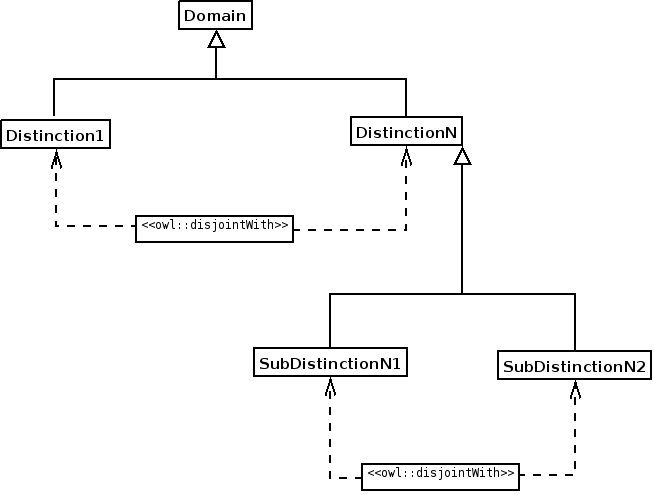
\includegraphics[width=\textwidth]{Catalogue/Upper_Level_Ontology_abstract}\caption{\label{odp:Upper_Level_Ontology_abstract} Abstract structure of the Upper Level Ontology ODP.}\end{figure}

\item [SAMPLE:] See Figure \ref{odp:Upper_Level_Ontology_instance}.
\begin{figure}[]\centering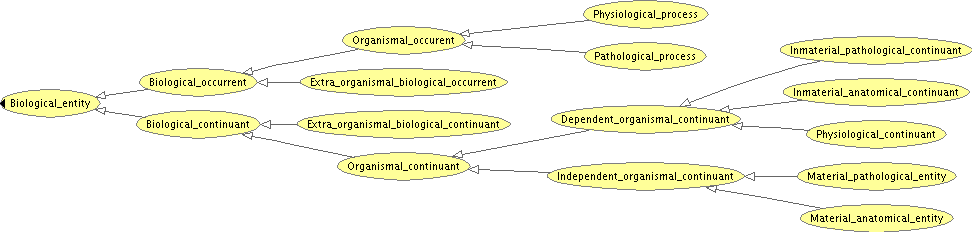
\includegraphics[width=\textwidth]{Catalogue/Upper_Level_Ontology_instance}\caption{\label{odp:Upper_Level_Ontology_instance} Sample structure of the Upper Level Ontology ODP.}\end{figure}

\item [ELEMENTS:] All the classes that represent a conceptual category.

\item [IMPLEMENTATION:] The different hierarchies of primitive classes must be asserted using disjoints.

\item [RESULT:] By endorsing to a given Upper Level Ontology when building a domain ontology the ontologists makes the integration of the ontology with other ontologies a much easier process. Besides, the ontology becomes a cleaner model with different modules.

\item [SIDE EFFECTS:] The ontology is committed to a concrete view of the knowledge domain (given by the Upper Level Ontology), and therefore the use and implantation of Upper Level Ontologies is very controversial.

\item [REFERENCES: ] ~\begin{itemize}
\item Barry Smith et al. A Strategy for Improving and Integrating Biomedical Ontologies. AMIA 2005.
\item \url{http://www.co-ode.org/resources/tutorials/bio/}\end{itemize}
\item [URL: ] \url{http://www.gong.manchester.ac.uk/odp/owl/Good_Practice_ODP/Upper_Level_Ontology.owl} \end{description}